% Mobile Ansicht „Quotes -> Gold antippen“: aufgeklappte Angaben eines Instruments
% (blaues Design) – Vektor-Nachbau.
% Grundlage: DOM-Messung originals/messungen/instrument-info-mobil.json (Fenster 440 px
% breit, Inter). Alle Maße in CSS-px, Ursprung oben links am .accordion-item, y nach unten.
% Bild = der gemessene Block, 410 x 327,2 px.
%
% Gemessen:
%   .accordion-item  410 x 327,2, Radius 3 px, Fläche rgba(14,80,114,0.1), Inter 12 px
%   Kopfzeile        <button> 410 x 40, flex, padding 0 5px, line-height 20 px, Text weiß 400
%     i.icon-star    x10 y13 14 x 14, icomoon 14 px, rgb(91,106,130), Glyphe U+E916
%                    – WEGGELASSEN: nicht in icons.tikz, Plattform-Schrift nicht verfügbar
%     img.flag       x46 y14,1 22 x 14, assets/images/instruments/XAUUSD.png
%                    – WEGGELASSEN (Rasterbild), Fläche bleibt leer
%     span „Gold“    x77 y10 112 x 20, padding 0 5px, text-align center, weiß
%     span Bid       x189 y10 92 x 20, padding 0 5px, center, rgb(83,188,81) (color-green-main)
%     span Ask       x281 y10 92 x 20, padding 0 5px, center, weiß (color00)
%     i.icon-arrow-down  x383 y14 12 x 12, icomoon 12 px, weiß, Glyphe U+E910
%                    – WEGGELASSEN: nicht in icons.tikz, Plattform-Schrift nicht verfügbar
%   .accordion-body  x0 y40 410 x 287,2, Fläche rgb(4,39,60), padding 16px 10px
%     Raster 3 Spalten je 119,3 px bei x 10 / 145,3 / 280,7 (Abstand 16 px);
%     Zeilen bei y 56 / 101 / 146 / 191, je 29 px hoch (Abstand 16 px).
%     Zelle: span.ttl (Titel) 14 px hoch, margin-bottom 1 px, rgb(168,187,190);
%            darunter der Wert als Text, line-height 14 px, weiß. Beide 12 px, 400.
%     Schaltflächen a.button: 189 x 29,6 px, Radius 5 px, Rahmen 0,8 px (Farbe nicht in
%       der Messung, wie bei anderen Default-Werten vermutlich transparent -> als volle
%       Fläche gezeichnet), padding 6px 10px; Text 12 px, 600, line-height 16 px, weiß,
%       zentriert. x 10 / 211, y 240 / 281,6; Flächen:
%       New order rgb(83,188,81), New pending order rgb(249,64,86),
%       New chart rgb(14,80,114), Trade Hours rgb(6,47,71).
%
% Kopfzeile: rgba(14,80,114,0.1) über dem Seitenhintergrund. Der Seitenhintergrund ist in
% der Messung nicht enthalten; wie in mobil.tex gilt #04273C (Fläche unter den Reitern =
% panel.pdf). Mischfarbe 0,1 * (14,80,114) + 0,9 * (4,39,60) = (5,0; 43,1; 65,4)
% -> rgb(5,43,65). Der Körper rgb(4,39,60) gleicht dem Seitenhintergrund; die Ecken des
% Ausschnitts folgen daher dem Radius 3 px des .accordion-item.
%
% Grundlinien: Inter 4.0, Ascent 1984, Descent 494 (unitsPerEm 2048). Bei line-height L
% liegt die Grundlinie L/2 + (1984-494)/4096 em unter der Oberkante der Zeile, bei 12 px
% also L/2 + 4,365 px (Chrome rundet Ascent/Descent in Gerätepixeln; Abweichung < 0,1 px).
%
% Abweichungen vom Original (Regeln des Nutzers): keine Zahlen und kein „Bid“/„Ask“ ->
% die Werte sind kurze Wörter (Liste \angaben unten, wie info-desktop.tex; Commission „—“
% wie Bonus/Credit in bar.tex), die beiden Kurse heißen „Kurs“.
%
% Marken (Schalter \ifmarken, Standard: an): weiße Kreise mit Nummer wie in panel.pdf
% (Radius 11 px, Inter SemiBold 12 px in #04273C, Grundlinie 4 px unter der Mitte), 25 px rechts hinter dem Titel, mittig
% zur Titelzeile: 1 Swap long, 2 Swap short, 3 Leverage:.
% Ohne Marken bauen: xelatex -jobname=info-mobil-ohne '\def\ohnemarken{}% Mobile Ansicht „Quotes -> Gold antippen“: aufgeklappte Angaben eines Instruments
% (blaues Design) – Vektor-Nachbau.
% Grundlage: DOM-Messung originals/messungen/instrument-info-mobil.json (Fenster 440 px
% breit, Inter). Alle Maße in CSS-px, Ursprung oben links am .accordion-item, y nach unten.
% Bild = der gemessene Block, 410 x 327,2 px.
%
% Gemessen:
%   .accordion-item  410 x 327,2, Radius 3 px, Fläche rgba(14,80,114,0.1), Inter 12 px
%   Kopfzeile        <button> 410 x 40, flex, padding 0 5px, line-height 20 px, Text weiß 400
%     i.icon-star    x10 y13 14 x 14, icomoon 14 px, rgb(91,106,130), Glyphe U+E916
%                    – WEGGELASSEN: nicht in icons.tikz, Plattform-Schrift nicht verfügbar
%     img.flag       x46 y14,1 22 x 14, assets/images/instruments/XAUUSD.png
%                    – WEGGELASSEN (Rasterbild), Fläche bleibt leer
%     span „Gold“    x77 y10 112 x 20, padding 0 5px, text-align center, weiß
%     span Bid       x189 y10 92 x 20, padding 0 5px, center, rgb(83,188,81) (color-green-main)
%     span Ask       x281 y10 92 x 20, padding 0 5px, center, weiß (color00)
%     i.icon-arrow-down  x383 y14 12 x 12, icomoon 12 px, weiß, Glyphe U+E910
%                    – WEGGELASSEN: nicht in icons.tikz, Plattform-Schrift nicht verfügbar
%   .accordion-body  x0 y40 410 x 287,2, Fläche rgb(4,39,60), padding 16px 10px
%     Raster 3 Spalten je 119,3 px bei x 10 / 145,3 / 280,7 (Abstand 16 px);
%     Zeilen bei y 56 / 101 / 146 / 191, je 29 px hoch (Abstand 16 px).
%     Zelle: span.ttl (Titel) 14 px hoch, margin-bottom 1 px, rgb(168,187,190);
%            darunter der Wert als Text, line-height 14 px, weiß. Beide 12 px, 400.
%     Schaltflächen a.button: 189 x 29,6 px, Radius 5 px, Rahmen 0,8 px (Farbe nicht in
%       der Messung, wie bei anderen Default-Werten vermutlich transparent -> als volle
%       Fläche gezeichnet), padding 6px 10px; Text 12 px, 600, line-height 16 px, weiß,
%       zentriert. x 10 / 211, y 240 / 281,6; Flächen:
%       New order rgb(83,188,81), New pending order rgb(249,64,86),
%       New chart rgb(14,80,114), Trade Hours rgb(6,47,71).
%
% Kopfzeile: rgba(14,80,114,0.1) über dem Seitenhintergrund. Der Seitenhintergrund ist in
% der Messung nicht enthalten; wie in mobil.tex gilt #04273C (Fläche unter den Reitern =
% panel.pdf). Mischfarbe 0,1 * (14,80,114) + 0,9 * (4,39,60) = (5,0; 43,1; 65,4)
% -> rgb(5,43,65). Der Körper rgb(4,39,60) gleicht dem Seitenhintergrund; die Ecken des
% Ausschnitts folgen daher dem Radius 3 px des .accordion-item.
%
% Grundlinien: Inter 4.0, Ascent 1984, Descent 494 (unitsPerEm 2048). Bei line-height L
% liegt die Grundlinie L/2 + (1984-494)/4096 em unter der Oberkante der Zeile, bei 12 px
% also L/2 + 4,365 px (Chrome rundet Ascent/Descent in Gerätepixeln; Abweichung < 0,1 px).
%
% Abweichungen vom Original (Regeln des Nutzers): keine Zahlen und kein „Bid“/„Ask“ ->
% die Werte sind kurze Wörter (Liste \angaben unten, wie info-desktop.tex; Commission „—“
% wie Bonus/Credit in bar.tex), die beiden Kurse heißen „Kurs“.
%
% Marken (Schalter \ifmarken, Standard: an): weiße Kreise mit Nummer wie in panel.pdf
% (Radius 11 px, Inter SemiBold 12 px in #04273C, Grundlinie 4 px unter der Mitte), 25 px rechts hinter dem Titel, mittig
% zur Titelzeile: 1 Swap long, 2 Swap short, 3 Leverage:.
% Ohne Marken bauen: xelatex -jobname=info-mobil-ohne '\def\ohnemarken{}% Mobile Ansicht „Quotes -> Gold antippen“: aufgeklappte Angaben eines Instruments
% (blaues Design) – Vektor-Nachbau.
% Grundlage: DOM-Messung originals/messungen/instrument-info-mobil.json (Fenster 440 px
% breit, Inter). Alle Maße in CSS-px, Ursprung oben links am .accordion-item, y nach unten.
% Bild = der gemessene Block, 410 x 327,2 px.
%
% Gemessen:
%   .accordion-item  410 x 327,2, Radius 3 px, Fläche rgba(14,80,114,0.1), Inter 12 px
%   Kopfzeile        <button> 410 x 40, flex, padding 0 5px, line-height 20 px, Text weiß 400
%     i.icon-star    x10 y13 14 x 14, icomoon 14 px, rgb(91,106,130), Glyphe U+E916
%                    – WEGGELASSEN: nicht in icons.tikz, Plattform-Schrift nicht verfügbar
%     img.flag       x46 y14,1 22 x 14, assets/images/instruments/XAUUSD.png
%                    – WEGGELASSEN (Rasterbild), Fläche bleibt leer
%     span „Gold“    x77 y10 112 x 20, padding 0 5px, text-align center, weiß
%     span Bid       x189 y10 92 x 20, padding 0 5px, center, rgb(83,188,81) (color-green-main)
%     span Ask       x281 y10 92 x 20, padding 0 5px, center, weiß (color00)
%     i.icon-arrow-down  x383 y14 12 x 12, icomoon 12 px, weiß, Glyphe U+E910
%                    – WEGGELASSEN: nicht in icons.tikz, Plattform-Schrift nicht verfügbar
%   .accordion-body  x0 y40 410 x 287,2, Fläche rgb(4,39,60), padding 16px 10px
%     Raster 3 Spalten je 119,3 px bei x 10 / 145,3 / 280,7 (Abstand 16 px);
%     Zeilen bei y 56 / 101 / 146 / 191, je 29 px hoch (Abstand 16 px).
%     Zelle: span.ttl (Titel) 14 px hoch, margin-bottom 1 px, rgb(168,187,190);
%            darunter der Wert als Text, line-height 14 px, weiß. Beide 12 px, 400.
%     Schaltflächen a.button: 189 x 29,6 px, Radius 5 px, Rahmen 0,8 px (Farbe nicht in
%       der Messung, wie bei anderen Default-Werten vermutlich transparent -> als volle
%       Fläche gezeichnet), padding 6px 10px; Text 12 px, 600, line-height 16 px, weiß,
%       zentriert. x 10 / 211, y 240 / 281,6; Flächen:
%       New order rgb(83,188,81), New pending order rgb(249,64,86),
%       New chart rgb(14,80,114), Trade Hours rgb(6,47,71).
%
% Kopfzeile: rgba(14,80,114,0.1) über dem Seitenhintergrund. Der Seitenhintergrund ist in
% der Messung nicht enthalten; wie in mobil.tex gilt #04273C (Fläche unter den Reitern =
% panel.pdf). Mischfarbe 0,1 * (14,80,114) + 0,9 * (4,39,60) = (5,0; 43,1; 65,4)
% -> rgb(5,43,65). Der Körper rgb(4,39,60) gleicht dem Seitenhintergrund; die Ecken des
% Ausschnitts folgen daher dem Radius 3 px des .accordion-item.
%
% Grundlinien: Inter 4.0, Ascent 1984, Descent 494 (unitsPerEm 2048). Bei line-height L
% liegt die Grundlinie L/2 + (1984-494)/4096 em unter der Oberkante der Zeile, bei 12 px
% also L/2 + 4,365 px (Chrome rundet Ascent/Descent in Gerätepixeln; Abweichung < 0,1 px).
%
% Abweichungen vom Original (Regeln des Nutzers): keine Zahlen und kein „Bid“/„Ask“ ->
% die Werte sind kurze Wörter (Liste \angaben unten, wie info-desktop.tex; Commission „—“
% wie Bonus/Credit in bar.tex), die beiden Kurse heißen „Kurs“.
%
% Marken (Schalter \ifmarken, Standard: an): weiße Kreise mit Nummer wie in panel.pdf
% (Radius 11 px, Inter SemiBold 12 px in #04273C, Grundlinie 4 px unter der Mitte), 25 px rechts hinter dem Titel, mittig
% zur Titelzeile: 1 Swap long, 2 Swap short, 3 Leverage:.
% Ohne Marken bauen: xelatex -jobname=info-mobil-ohne '\def\ohnemarken{}% Mobile Ansicht „Quotes -> Gold antippen“: aufgeklappte Angaben eines Instruments
% (blaues Design) – Vektor-Nachbau.
% Grundlage: DOM-Messung originals/messungen/instrument-info-mobil.json (Fenster 440 px
% breit, Inter). Alle Maße in CSS-px, Ursprung oben links am .accordion-item, y nach unten.
% Bild = der gemessene Block, 410 x 327,2 px.
%
% Gemessen:
%   .accordion-item  410 x 327,2, Radius 3 px, Fläche rgba(14,80,114,0.1), Inter 12 px
%   Kopfzeile        <button> 410 x 40, flex, padding 0 5px, line-height 20 px, Text weiß 400
%     i.icon-star    x10 y13 14 x 14, icomoon 14 px, rgb(91,106,130), Glyphe U+E916
%                    – WEGGELASSEN: nicht in icons.tikz, Plattform-Schrift nicht verfügbar
%     img.flag       x46 y14,1 22 x 14, assets/images/instruments/XAUUSD.png
%                    – WEGGELASSEN (Rasterbild), Fläche bleibt leer
%     span „Gold“    x77 y10 112 x 20, padding 0 5px, text-align center, weiß
%     span Bid       x189 y10 92 x 20, padding 0 5px, center, rgb(83,188,81) (color-green-main)
%     span Ask       x281 y10 92 x 20, padding 0 5px, center, weiß (color00)
%     i.icon-arrow-down  x383 y14 12 x 12, icomoon 12 px, weiß, Glyphe U+E910
%                    – WEGGELASSEN: nicht in icons.tikz, Plattform-Schrift nicht verfügbar
%   .accordion-body  x0 y40 410 x 287,2, Fläche rgb(4,39,60), padding 16px 10px
%     Raster 3 Spalten je 119,3 px bei x 10 / 145,3 / 280,7 (Abstand 16 px);
%     Zeilen bei y 56 / 101 / 146 / 191, je 29 px hoch (Abstand 16 px).
%     Zelle: span.ttl (Titel) 14 px hoch, margin-bottom 1 px, rgb(168,187,190);
%            darunter der Wert als Text, line-height 14 px, weiß. Beide 12 px, 400.
%     Schaltflächen a.button: 189 x 29,6 px, Radius 5 px, Rahmen 0,8 px (Farbe nicht in
%       der Messung, wie bei anderen Default-Werten vermutlich transparent -> als volle
%       Fläche gezeichnet), padding 6px 10px; Text 12 px, 600, line-height 16 px, weiß,
%       zentriert. x 10 / 211, y 240 / 281,6; Flächen:
%       New order rgb(83,188,81), New pending order rgb(249,64,86),
%       New chart rgb(14,80,114), Trade Hours rgb(6,47,71).
%
% Kopfzeile: rgba(14,80,114,0.1) über dem Seitenhintergrund. Der Seitenhintergrund ist in
% der Messung nicht enthalten; wie in mobil.tex gilt #04273C (Fläche unter den Reitern =
% panel.pdf). Mischfarbe 0,1 * (14,80,114) + 0,9 * (4,39,60) = (5,0; 43,1; 65,4)
% -> rgb(5,43,65). Der Körper rgb(4,39,60) gleicht dem Seitenhintergrund; die Ecken des
% Ausschnitts folgen daher dem Radius 3 px des .accordion-item.
%
% Grundlinien: Inter 4.0, Ascent 1984, Descent 494 (unitsPerEm 2048). Bei line-height L
% liegt die Grundlinie L/2 + (1984-494)/4096 em unter der Oberkante der Zeile, bei 12 px
% also L/2 + 4,365 px (Chrome rundet Ascent/Descent in Gerätepixeln; Abweichung < 0,1 px).
%
% Abweichungen vom Original (Regeln des Nutzers): keine Zahlen und kein „Bid“/„Ask“ ->
% die Werte sind kurze Wörter (Liste \angaben unten, wie info-desktop.tex; Commission „—“
% wie Bonus/Credit in bar.tex), die beiden Kurse heißen „Kurs“.
%
% Marken (Schalter \ifmarken, Standard: an): weiße Kreise mit Nummer wie in panel.pdf
% (Radius 11 px, Inter SemiBold 12 px in #04273C, Grundlinie 4 px unter der Mitte), 25 px rechts hinter dem Titel, mittig
% zur Titelzeile: 1 Swap long, 2 Swap short, 3 Leverage:.
% Ohne Marken bauen: xelatex -jobname=info-mobil-ohne '\def\ohnemarken{}\input{info-mobil}'
\documentclass[border=0pt]{standalone}
\usepackage{fontspec}
\usepackage{tikz}
\setmainfont{Inter}% Inter 4.0 Regular (Paket fonts-inter), wie bar.tex/mobil.tex
\newfontface\halbfett{Inter SemiBold}% font-weight 600

\newif\ifmarken \markentrue
\ifdefined\ohnemarken \markenfalse \fi

\newlength\px \setlength\px{0.75bp}% 1 CSS-px
\newcommand\schrift{\fontsize{9bp}{10.5bp}\selectfont}% 12 px
\definecolor{kopfzeile}{RGB}{5,43,65}%   rgba(14,80,114,0.1) über #04273C
\definecolor{koerper}{RGB}{4,39,60}%     .accordion-body
\definecolor{titel}{RGB}{168,187,190}%   span.ttl
\definecolor{gruen}{RGB}{83,188,81}%     color-green-main (Kurs links)
\definecolor{knopfa}{RGB}{83,188,81}%    New order
\definecolor{knopfb}{RGB}{249,64,86}%    New pending order
\definecolor{knopfc}{RGB}{14,80,114}%    New chart
\definecolor{knopfd}{RGB}{6,47,71}%      Trade Hours
\definecolor{markentext}{HTML}{04273C}%  Nummer in der Marke (wie panel.pdf)

\newcommand\breite{410}
\newcommand\hoehe{327.2}
\newcommand\gl{4.3652}% (1984-494)/4096 * 12 px

% Raster der Angaben: \zelle{<x>}{<y>}{<Titel>}{<Wert>}
\newcommand\angaben{%
  \zelle{10}{56}{Symbol}{Gold}%
  \zelle{145.3}{56}{Swap long}{Satz long}%
  \zelle{280.7}{56}{Swap short}{Satz short}%
  \zelle{10}{101}{Type}{Metals}%
  \zelle{145.3}{101}{Spread}{Wert}%
  \zelle{280.7}{101}{Gap Level}{Wert}%
  \zelle{10}{146}{Digits}{Stellen}%
  \zelle{145.3}{146}{Stop Level}{Wert}%
  \zelle{280.7}{146}{Commission}{—}%
  \zelle{10}{191}{Contract size:}{Größe}%
  \zelle{145.3}{191}{Leverage:}{Hebel}%
}
\newcommand\zelle[4]{%
  \node[anchor=base west,text=titel] at (#1,-#2-7-\gl) {#3};%      Titelzeile y .. y+14
  \node[anchor=base west,text=white] at (#1,-#2-15-7-\gl) {#4};}%  Wertzeile y+15 .. y+29

% Schaltflächen: \knopf{<x>}{<y>}{<Farbe>}{<Text>}
\newcommand\knopf[4]{%
  \fill[#3,rounded corners=5\px] (#1,-#2) rectangle ++(189,-29.6);
  \node[anchor=base,text=white,font=\schrift\halbfett]
    at (#1+94.5,-#2-0.8-6-8-\gl) {#4};}

% Marken: Abstand vom Ende des Titels bis zum Kreisrand 25 px wie in panel.pdf.
% Titelbreiten vor dem Bild messen (im Bild schaltet TikZ auf \nullfont).
\newlength\tw
\makeatletter
\newcommand\titelende[3]{% {Name}{x}{Titel}
  \settowidth\tw{\schrift #3}%
  \expandafter\xdef\csname marke#1\endcsname{\strip@pt\dimexpr #2pt+\tw*4/3*7200/7227\relax}}
\titelende{a}{145.3}{Swap long}
\titelende{b}{280.7}{Swap short}
\titelende{c}{145.3}{Leverage:}
\titelende{sym}{10}{Symbol}\titelende{typ}{10}{Type}\titelende{dig}{10}{Digits}
\titelende{con}{10}{Contract size:}\titelende{spr}{145.3}{Spread}\titelende{sto}{145.3}{Stop Level}
\titelende{gap}{280.7}{Gap Level}\titelende{com}{280.7}{Commission}
\makeatother
% \knopfmarke{<x>}{<y>}{<Nummer>}: Marke links in der Schaltfläche (Mitte 19 px vom Rand)
\newcommand\knopfmarke[3]{%
  \fill[white] (#1+19,-#2-14.8) circle[radius=11];
  \node[anchor=base,text=markentext,font=\schrift\halbfett] at (#1+19,-#2-14.8-4) {#3};}
\newcommand\marke[3]{% {Ende des Titels in px}{y der Zelle}{Nummer}
  \fill[white] (#1+25+11,-#2-7) circle[radius=11];
  \node[anchor=base,text=markentext,font=\schrift\halbfett] at (#1+25+11,-#2-7-4) {#3};}

% Kontrolle: Textbreiten der Schaltflächen (gemessen 60,3 / 110,7 / 59,6 / 71,4 px)
\newcommand\breitepx[1]{\settowidth\tw{\schrift\halbfett #1}%
  \typeout{INFO-MOBIL: Breite '#1' \the\dimexpr\tw*4/3*7200/7227\relax\space(in px)}}
\breitepx{New order}\breitepx{New pending order}\breitepx{New chart}\breitepx{Trade Hours}
\typeout{INFO-MOBIL: Titelende Swap long \markea, Swap short \markeb, Leverage: \markec\space px}

\begin{document}%
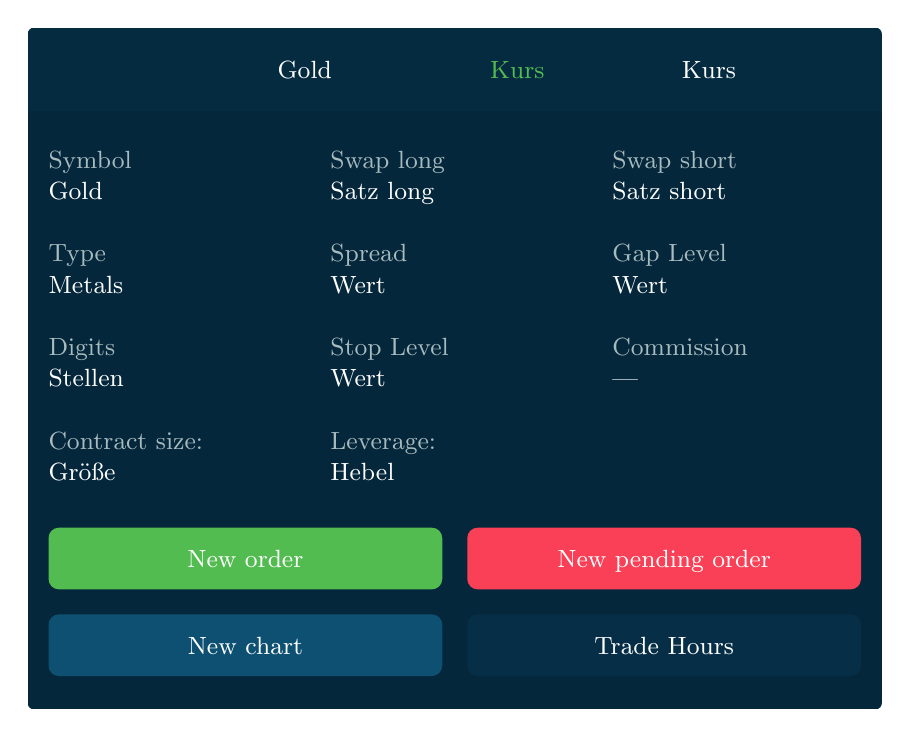
\begin{tikzpicture}[x=\px,y=\px,font=\schrift,every node/.style={inner sep=0,outer sep=0}]
  \path[use as bounding box] (0,0) rectangle (\breite,-\hoehe);
  \clip[rounded corners=3\px] (0,0) rectangle (\breite,-\hoehe);
  % Kopfzeile (Stern, Bild und Aufklapp-Pfeil weggelassen, siehe oben)
  \fill[kopfzeile] (0,0) rectangle (\breite,-40);
  \node[anchor=base,text=white] at (133,-10-10-\gl) {Gold};%  Inhalt 82..184
  \node[anchor=base,text=gruen] at (235,-10-10-\gl) {Kurs};%  Inhalt 194..276
  \node[anchor=base,text=white] at (327,-10-10-\gl) {Kurs};%  Inhalt 286..368
  % Angaben
  \fill[koerper] (0,-40) rectangle (\breite,-\hoehe);
  \angaben
  \knopf{10}{240}{knopfa}{New order}
  \knopf{211}{240}{knopfb}{New pending order}
  \knopf{10}{281.6}{knopfc}{New chart}
  \knopf{211}{281.6}{knopfd}{Trade Hours}
  \ifmarken% alle Angaben und Schaltflächen nummeriert (Nutzerwunsch 02.10.2026),
    % Nummern wie in info-desktop.tex
    \marke{\markesym}{56}{1}\marke{\markea}{56}{7}\marke{\markeb}{56}{8}
    \marke{\marketyp}{101}{2}\marke{\markespr}{101}{3}\marke{\markegap}{101}{10}
    \marke{\markedig}{146}{4}\marke{\markesto}{146}{11}\marke{\markecom}{146}{5}
    \marke{\markecon}{191}{6}\marke{\markec}{191}{9}
    \knopfmarke{10}{240}{12}\knopfmarke{211}{240}{13}
    \knopfmarke{10}{281.6}{14}\knopfmarke{211}{281.6}{15}
  \fi
\end{tikzpicture}%
\end{document}
'
\documentclass[border=0pt]{standalone}
\usepackage{fontspec}
\usepackage{tikz}
\setmainfont{Inter}% Inter 4.0 Regular (Paket fonts-inter), wie bar.tex/mobil.tex
\newfontface\halbfett{Inter SemiBold}% font-weight 600

\newif\ifmarken \markentrue
\ifdefined\ohnemarken \markenfalse \fi

\newlength\px \setlength\px{0.75bp}% 1 CSS-px
\newcommand\schrift{\fontsize{9bp}{10.5bp}\selectfont}% 12 px
\definecolor{kopfzeile}{RGB}{5,43,65}%   rgba(14,80,114,0.1) über #04273C
\definecolor{koerper}{RGB}{4,39,60}%     .accordion-body
\definecolor{titel}{RGB}{168,187,190}%   span.ttl
\definecolor{gruen}{RGB}{83,188,81}%     color-green-main (Kurs links)
\definecolor{knopfa}{RGB}{83,188,81}%    New order
\definecolor{knopfb}{RGB}{249,64,86}%    New pending order
\definecolor{knopfc}{RGB}{14,80,114}%    New chart
\definecolor{knopfd}{RGB}{6,47,71}%      Trade Hours
\definecolor{markentext}{HTML}{04273C}%  Nummer in der Marke (wie panel.pdf)

\newcommand\breite{410}
\newcommand\hoehe{327.2}
\newcommand\gl{4.3652}% (1984-494)/4096 * 12 px

% Raster der Angaben: \zelle{<x>}{<y>}{<Titel>}{<Wert>}
\newcommand\angaben{%
  \zelle{10}{56}{Symbol}{Gold}%
  \zelle{145.3}{56}{Swap long}{Satz long}%
  \zelle{280.7}{56}{Swap short}{Satz short}%
  \zelle{10}{101}{Type}{Metals}%
  \zelle{145.3}{101}{Spread}{Wert}%
  \zelle{280.7}{101}{Gap Level}{Wert}%
  \zelle{10}{146}{Digits}{Stellen}%
  \zelle{145.3}{146}{Stop Level}{Wert}%
  \zelle{280.7}{146}{Commission}{—}%
  \zelle{10}{191}{Contract size:}{Größe}%
  \zelle{145.3}{191}{Leverage:}{Hebel}%
}
\newcommand\zelle[4]{%
  \node[anchor=base west,text=titel] at (#1,-#2-7-\gl) {#3};%      Titelzeile y .. y+14
  \node[anchor=base west,text=white] at (#1,-#2-15-7-\gl) {#4};}%  Wertzeile y+15 .. y+29

% Schaltflächen: \knopf{<x>}{<y>}{<Farbe>}{<Text>}
\newcommand\knopf[4]{%
  \fill[#3,rounded corners=5\px] (#1,-#2) rectangle ++(189,-29.6);
  \node[anchor=base,text=white,font=\schrift\halbfett]
    at (#1+94.5,-#2-0.8-6-8-\gl) {#4};}

% Marken: Abstand vom Ende des Titels bis zum Kreisrand 25 px wie in panel.pdf.
% Titelbreiten vor dem Bild messen (im Bild schaltet TikZ auf \nullfont).
\newlength\tw
\makeatletter
\newcommand\titelende[3]{% {Name}{x}{Titel}
  \settowidth\tw{\schrift #3}%
  \expandafter\xdef\csname marke#1\endcsname{\strip@pt\dimexpr #2pt+\tw*4/3*7200/7227\relax}}
\titelende{a}{145.3}{Swap long}
\titelende{b}{280.7}{Swap short}
\titelende{c}{145.3}{Leverage:}
\titelende{sym}{10}{Symbol}\titelende{typ}{10}{Type}\titelende{dig}{10}{Digits}
\titelende{con}{10}{Contract size:}\titelende{spr}{145.3}{Spread}\titelende{sto}{145.3}{Stop Level}
\titelende{gap}{280.7}{Gap Level}\titelende{com}{280.7}{Commission}
\makeatother
% \knopfmarke{<x>}{<y>}{<Nummer>}: Marke links in der Schaltfläche (Mitte 19 px vom Rand)
\newcommand\knopfmarke[3]{%
  \fill[white] (#1+19,-#2-14.8) circle[radius=11];
  \node[anchor=base,text=markentext,font=\schrift\halbfett] at (#1+19,-#2-14.8-4) {#3};}
\newcommand\marke[3]{% {Ende des Titels in px}{y der Zelle}{Nummer}
  \fill[white] (#1+25+11,-#2-7) circle[radius=11];
  \node[anchor=base,text=markentext,font=\schrift\halbfett] at (#1+25+11,-#2-7-4) {#3};}

% Kontrolle: Textbreiten der Schaltflächen (gemessen 60,3 / 110,7 / 59,6 / 71,4 px)
\newcommand\breitepx[1]{\settowidth\tw{\schrift\halbfett #1}%
  \typeout{INFO-MOBIL: Breite '#1' \the\dimexpr\tw*4/3*7200/7227\relax\space(in px)}}
\breitepx{New order}\breitepx{New pending order}\breitepx{New chart}\breitepx{Trade Hours}
\typeout{INFO-MOBIL: Titelende Swap long \markea, Swap short \markeb, Leverage: \markec\space px}

\begin{document}%
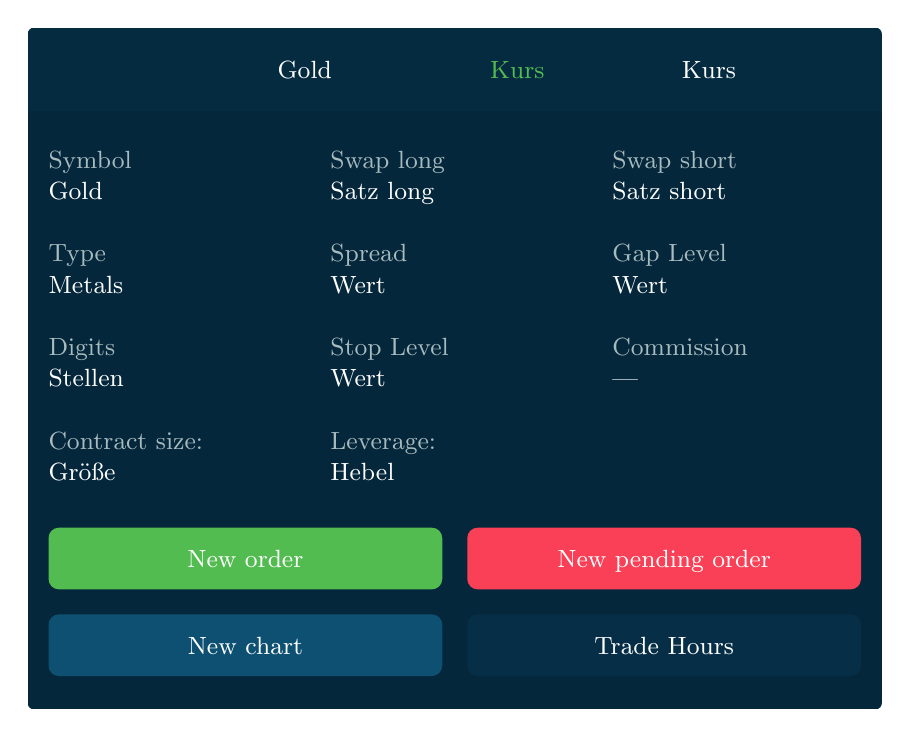
\begin{tikzpicture}[x=\px,y=\px,font=\schrift,every node/.style={inner sep=0,outer sep=0}]
  \path[use as bounding box] (0,0) rectangle (\breite,-\hoehe);
  \clip[rounded corners=3\px] (0,0) rectangle (\breite,-\hoehe);
  % Kopfzeile (Stern, Bild und Aufklapp-Pfeil weggelassen, siehe oben)
  \fill[kopfzeile] (0,0) rectangle (\breite,-40);
  \node[anchor=base,text=white] at (133,-10-10-\gl) {Gold};%  Inhalt 82..184
  \node[anchor=base,text=gruen] at (235,-10-10-\gl) {Kurs};%  Inhalt 194..276
  \node[anchor=base,text=white] at (327,-10-10-\gl) {Kurs};%  Inhalt 286..368
  % Angaben
  \fill[koerper] (0,-40) rectangle (\breite,-\hoehe);
  \angaben
  \knopf{10}{240}{knopfa}{New order}
  \knopf{211}{240}{knopfb}{New pending order}
  \knopf{10}{281.6}{knopfc}{New chart}
  \knopf{211}{281.6}{knopfd}{Trade Hours}
  \ifmarken% alle Angaben und Schaltflächen nummeriert (Nutzerwunsch 02.10.2026),
    % Nummern wie in info-desktop.tex
    \marke{\markesym}{56}{1}\marke{\markea}{56}{7}\marke{\markeb}{56}{8}
    \marke{\marketyp}{101}{2}\marke{\markespr}{101}{3}\marke{\markegap}{101}{10}
    \marke{\markedig}{146}{4}\marke{\markesto}{146}{11}\marke{\markecom}{146}{5}
    \marke{\markecon}{191}{6}\marke{\markec}{191}{9}
    \knopfmarke{10}{240}{12}\knopfmarke{211}{240}{13}
    \knopfmarke{10}{281.6}{14}\knopfmarke{211}{281.6}{15}
  \fi
\end{tikzpicture}%
\end{document}
'
\documentclass[border=0pt]{standalone}
\usepackage{fontspec}
\usepackage{tikz}
\setmainfont{Inter}% Inter 4.0 Regular (Paket fonts-inter), wie bar.tex/mobil.tex
\newfontface\halbfett{Inter SemiBold}% font-weight 600

\newif\ifmarken \markentrue
\ifdefined\ohnemarken \markenfalse \fi

\newlength\px \setlength\px{0.75bp}% 1 CSS-px
\newcommand\schrift{\fontsize{9bp}{10.5bp}\selectfont}% 12 px
\definecolor{kopfzeile}{RGB}{5,43,65}%   rgba(14,80,114,0.1) über #04273C
\definecolor{koerper}{RGB}{4,39,60}%     .accordion-body
\definecolor{titel}{RGB}{168,187,190}%   span.ttl
\definecolor{gruen}{RGB}{83,188,81}%     color-green-main (Kurs links)
\definecolor{knopfa}{RGB}{83,188,81}%    New order
\definecolor{knopfb}{RGB}{249,64,86}%    New pending order
\definecolor{knopfc}{RGB}{14,80,114}%    New chart
\definecolor{knopfd}{RGB}{6,47,71}%      Trade Hours
\definecolor{markentext}{HTML}{04273C}%  Nummer in der Marke (wie panel.pdf)

\newcommand\breite{410}
\newcommand\hoehe{327.2}
\newcommand\gl{4.3652}% (1984-494)/4096 * 12 px

% Raster der Angaben: \zelle{<x>}{<y>}{<Titel>}{<Wert>}
\newcommand\angaben{%
  \zelle{10}{56}{Symbol}{Gold}%
  \zelle{145.3}{56}{Swap long}{Satz long}%
  \zelle{280.7}{56}{Swap short}{Satz short}%
  \zelle{10}{101}{Type}{Metals}%
  \zelle{145.3}{101}{Spread}{Wert}%
  \zelle{280.7}{101}{Gap Level}{Wert}%
  \zelle{10}{146}{Digits}{Stellen}%
  \zelle{145.3}{146}{Stop Level}{Wert}%
  \zelle{280.7}{146}{Commission}{—}%
  \zelle{10}{191}{Contract size:}{Größe}%
  \zelle{145.3}{191}{Leverage:}{Hebel}%
}
\newcommand\zelle[4]{%
  \node[anchor=base west,text=titel] at (#1,-#2-7-\gl) {#3};%      Titelzeile y .. y+14
  \node[anchor=base west,text=white] at (#1,-#2-15-7-\gl) {#4};}%  Wertzeile y+15 .. y+29

% Schaltflächen: \knopf{<x>}{<y>}{<Farbe>}{<Text>}
\newcommand\knopf[4]{%
  \fill[#3,rounded corners=5\px] (#1,-#2) rectangle ++(189,-29.6);
  \node[anchor=base,text=white,font=\schrift\halbfett]
    at (#1+94.5,-#2-0.8-6-8-\gl) {#4};}

% Marken: Abstand vom Ende des Titels bis zum Kreisrand 25 px wie in panel.pdf.
% Titelbreiten vor dem Bild messen (im Bild schaltet TikZ auf \nullfont).
\newlength\tw
\makeatletter
\newcommand\titelende[3]{% {Name}{x}{Titel}
  \settowidth\tw{\schrift #3}%
  \expandafter\xdef\csname marke#1\endcsname{\strip@pt\dimexpr #2pt+\tw*4/3*7200/7227\relax}}
\titelende{a}{145.3}{Swap long}
\titelende{b}{280.7}{Swap short}
\titelende{c}{145.3}{Leverage:}
\titelende{sym}{10}{Symbol}\titelende{typ}{10}{Type}\titelende{dig}{10}{Digits}
\titelende{con}{10}{Contract size:}\titelende{spr}{145.3}{Spread}\titelende{sto}{145.3}{Stop Level}
\titelende{gap}{280.7}{Gap Level}\titelende{com}{280.7}{Commission}
\makeatother
% \knopfmarke{<x>}{<y>}{<Nummer>}: Marke links in der Schaltfläche (Mitte 19 px vom Rand)
\newcommand\knopfmarke[3]{%
  \fill[white] (#1+19,-#2-14.8) circle[radius=11];
  \node[anchor=base,text=markentext,font=\schrift\halbfett] at (#1+19,-#2-14.8-4) {#3};}
\newcommand\marke[3]{% {Ende des Titels in px}{y der Zelle}{Nummer}
  \fill[white] (#1+25+11,-#2-7) circle[radius=11];
  \node[anchor=base,text=markentext,font=\schrift\halbfett] at (#1+25+11,-#2-7-4) {#3};}

% Kontrolle: Textbreiten der Schaltflächen (gemessen 60,3 / 110,7 / 59,6 / 71,4 px)
\newcommand\breitepx[1]{\settowidth\tw{\schrift\halbfett #1}%
  \typeout{INFO-MOBIL: Breite '#1' \the\dimexpr\tw*4/3*7200/7227\relax\space(in px)}}
\breitepx{New order}\breitepx{New pending order}\breitepx{New chart}\breitepx{Trade Hours}
\typeout{INFO-MOBIL: Titelende Swap long \markea, Swap short \markeb, Leverage: \markec\space px}

\begin{document}%
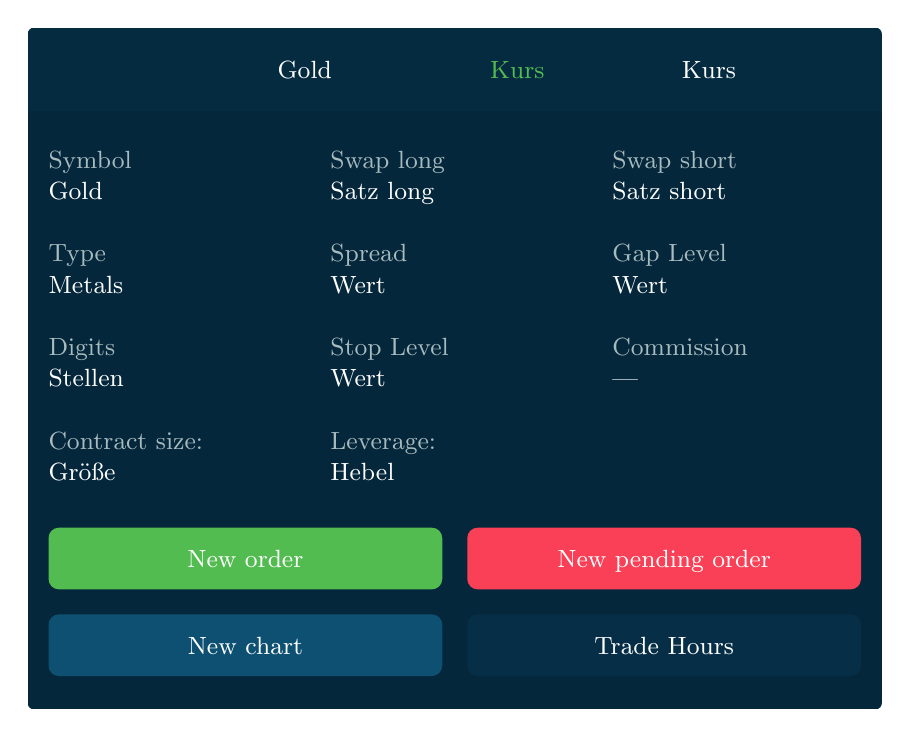
\begin{tikzpicture}[x=\px,y=\px,font=\schrift,every node/.style={inner sep=0,outer sep=0}]
  \path[use as bounding box] (0,0) rectangle (\breite,-\hoehe);
  \clip[rounded corners=3\px] (0,0) rectangle (\breite,-\hoehe);
  % Kopfzeile (Stern, Bild und Aufklapp-Pfeil weggelassen, siehe oben)
  \fill[kopfzeile] (0,0) rectangle (\breite,-40);
  \node[anchor=base,text=white] at (133,-10-10-\gl) {Gold};%  Inhalt 82..184
  \node[anchor=base,text=gruen] at (235,-10-10-\gl) {Kurs};%  Inhalt 194..276
  \node[anchor=base,text=white] at (327,-10-10-\gl) {Kurs};%  Inhalt 286..368
  % Angaben
  \fill[koerper] (0,-40) rectangle (\breite,-\hoehe);
  \angaben
  \knopf{10}{240}{knopfa}{New order}
  \knopf{211}{240}{knopfb}{New pending order}
  \knopf{10}{281.6}{knopfc}{New chart}
  \knopf{211}{281.6}{knopfd}{Trade Hours}
  \ifmarken% alle Angaben und Schaltflächen nummeriert (Nutzerwunsch 02.10.2026),
    % Nummern wie in info-desktop.tex
    \marke{\markesym}{56}{1}\marke{\markea}{56}{7}\marke{\markeb}{56}{8}
    \marke{\marketyp}{101}{2}\marke{\markespr}{101}{3}\marke{\markegap}{101}{10}
    \marke{\markedig}{146}{4}\marke{\markesto}{146}{11}\marke{\markecom}{146}{5}
    \marke{\markecon}{191}{6}\marke{\markec}{191}{9}
    \knopfmarke{10}{240}{12}\knopfmarke{211}{240}{13}
    \knopfmarke{10}{281.6}{14}\knopfmarke{211}{281.6}{15}
  \fi
\end{tikzpicture}%
\end{document}
'
\documentclass[border=0pt]{standalone}
\usepackage{fontspec}
\usepackage{tikz}
\setmainfont{Inter}% Inter 4.0 Regular (Paket fonts-inter), wie bar.tex/mobil.tex
\newfontface\halbfett{Inter SemiBold}% font-weight 600

\newif\ifmarken \markentrue
\ifdefined\ohnemarken \markenfalse \fi

\newlength\px \setlength\px{0.75bp}% 1 CSS-px
\newcommand\schrift{\fontsize{9bp}{10.5bp}\selectfont}% 12 px
\definecolor{kopfzeile}{RGB}{5,43,65}%   rgba(14,80,114,0.1) über #04273C
\definecolor{koerper}{RGB}{4,39,60}%     .accordion-body
\definecolor{titel}{RGB}{168,187,190}%   span.ttl
\definecolor{gruen}{RGB}{83,188,81}%     color-green-main (Kurs links)
\definecolor{knopfa}{RGB}{83,188,81}%    New order
\definecolor{knopfb}{RGB}{249,64,86}%    New pending order
\definecolor{knopfc}{RGB}{14,80,114}%    New chart
\definecolor{knopfd}{RGB}{6,47,71}%      Trade Hours
\definecolor{markentext}{HTML}{04273C}%  Nummer in der Marke (wie panel.pdf)

\newcommand\breite{410}
\newcommand\hoehe{327.2}
\newcommand\gl{4.3652}% (1984-494)/4096 * 12 px

% Raster der Angaben: \zelle{<x>}{<y>}{<Titel>}{<Wert>}
\newcommand\angaben{%
  \zelle{10}{56}{Symbol}{Gold}%
  \zelle{145.3}{56}{Swap long}{Satz long}%
  \zelle{280.7}{56}{Swap short}{Satz short}%
  \zelle{10}{101}{Type}{Metals}%
  \zelle{145.3}{101}{Spread}{Wert}%
  \zelle{280.7}{101}{Gap Level}{Wert}%
  \zelle{10}{146}{Digits}{Stellen}%
  \zelle{145.3}{146}{Stop Level}{Wert}%
  \zelle{280.7}{146}{Commission}{—}%
  \zelle{10}{191}{Contract size:}{Größe}%
  \zelle{145.3}{191}{Leverage:}{Hebel}%
}
\newcommand\zelle[4]{%
  \node[anchor=base west,text=titel] at (#1,-#2-7-\gl) {#3};%      Titelzeile y .. y+14
  \node[anchor=base west,text=white] at (#1,-#2-15-7-\gl) {#4};}%  Wertzeile y+15 .. y+29

% Schaltflächen: \knopf{<x>}{<y>}{<Farbe>}{<Text>}
\newcommand\knopf[4]{%
  \fill[#3,rounded corners=5\px] (#1,-#2) rectangle ++(189,-29.6);
  \node[anchor=base,text=white,font=\schrift\halbfett]
    at (#1+94.5,-#2-0.8-6-8-\gl) {#4};}

% Marken: Abstand vom Ende des Titels bis zum Kreisrand 25 px wie in panel.pdf.
% Titelbreiten vor dem Bild messen (im Bild schaltet TikZ auf \nullfont).
\newlength\tw
\makeatletter
\newcommand\titelende[3]{% {Name}{x}{Titel}
  \settowidth\tw{\schrift #3}%
  \expandafter\xdef\csname marke#1\endcsname{\strip@pt\dimexpr #2pt+\tw*4/3*7200/7227\relax}}
\titelende{a}{145.3}{Swap long}
\titelende{b}{280.7}{Swap short}
\titelende{c}{145.3}{Leverage:}
\titelende{sym}{10}{Symbol}\titelende{typ}{10}{Type}\titelende{dig}{10}{Digits}
\titelende{con}{10}{Contract size:}\titelende{spr}{145.3}{Spread}\titelende{sto}{145.3}{Stop Level}
\titelende{gap}{280.7}{Gap Level}\titelende{com}{280.7}{Commission}
\makeatother
% \knopfmarke{<x>}{<y>}{<Nummer>}: Marke links in der Schaltfläche (Mitte 19 px vom Rand)
\newcommand\knopfmarke[3]{%
  \fill[white] (#1+19,-#2-14.8) circle[radius=11];
  \node[anchor=base,text=markentext,font=\schrift\halbfett] at (#1+19,-#2-14.8-4) {#3};}
\newcommand\marke[3]{% {Ende des Titels in px}{y der Zelle}{Nummer}
  \fill[white] (#1+25+11,-#2-7) circle[radius=11];
  \node[anchor=base,text=markentext,font=\schrift\halbfett] at (#1+25+11,-#2-7-4) {#3};}

% Kontrolle: Textbreiten der Schaltflächen (gemessen 60,3 / 110,7 / 59,6 / 71,4 px)
\newcommand\breitepx[1]{\settowidth\tw{\schrift\halbfett #1}%
  \typeout{INFO-MOBIL: Breite '#1' \the\dimexpr\tw*4/3*7200/7227\relax\space(in px)}}
\breitepx{New order}\breitepx{New pending order}\breitepx{New chart}\breitepx{Trade Hours}
\typeout{INFO-MOBIL: Titelende Swap long \markea, Swap short \markeb, Leverage: \markec\space px}

\begin{document}%
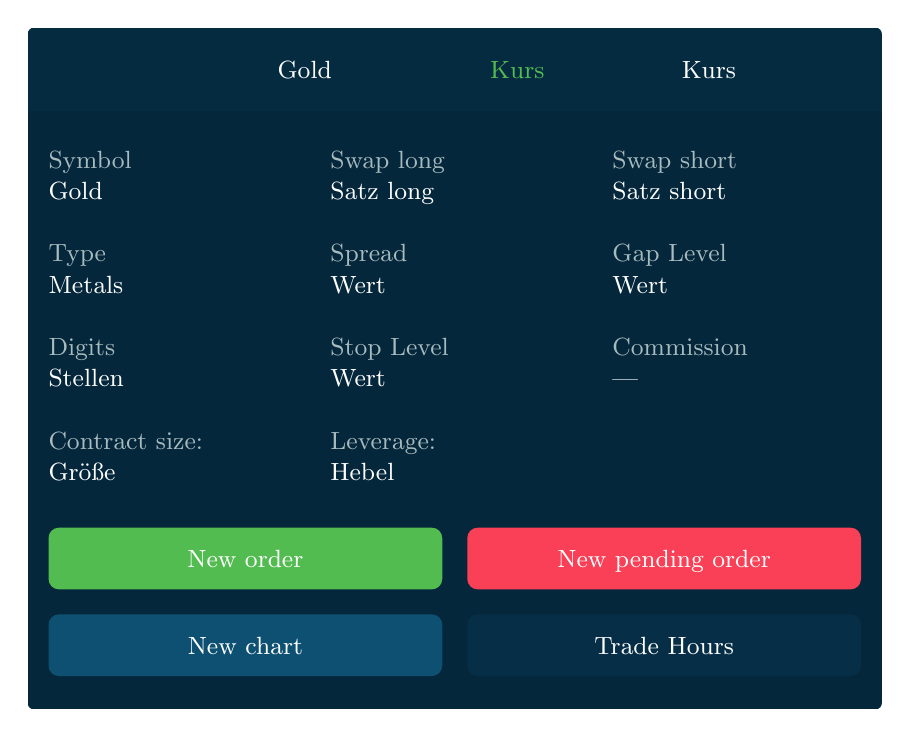
\begin{tikzpicture}[x=\px,y=\px,font=\schrift,every node/.style={inner sep=0,outer sep=0}]
  \path[use as bounding box] (0,0) rectangle (\breite,-\hoehe);
  \clip[rounded corners=3\px] (0,0) rectangle (\breite,-\hoehe);
  % Kopfzeile (Stern, Bild und Aufklapp-Pfeil weggelassen, siehe oben)
  \fill[kopfzeile] (0,0) rectangle (\breite,-40);
  \node[anchor=base,text=white] at (133,-10-10-\gl) {Gold};%  Inhalt 82..184
  \node[anchor=base,text=gruen] at (235,-10-10-\gl) {Kurs};%  Inhalt 194..276
  \node[anchor=base,text=white] at (327,-10-10-\gl) {Kurs};%  Inhalt 286..368
  % Angaben
  \fill[koerper] (0,-40) rectangle (\breite,-\hoehe);
  \angaben
  \knopf{10}{240}{knopfa}{New order}
  \knopf{211}{240}{knopfb}{New pending order}
  \knopf{10}{281.6}{knopfc}{New chart}
  \knopf{211}{281.6}{knopfd}{Trade Hours}
  \ifmarken% alle Angaben und Schaltflächen nummeriert (Nutzerwunsch 02.10.2026),
    % Nummern wie in info-desktop.tex
    \marke{\markesym}{56}{1}\marke{\markea}{56}{7}\marke{\markeb}{56}{8}
    \marke{\marketyp}{101}{2}\marke{\markespr}{101}{3}\marke{\markegap}{101}{10}
    \marke{\markedig}{146}{4}\marke{\markesto}{146}{11}\marke{\markecom}{146}{5}
    \marke{\markecon}{191}{6}\marke{\markec}{191}{9}
    \knopfmarke{10}{240}{12}\knopfmarke{211}{240}{13}
    \knopfmarke{10}{281.6}{14}\knopfmarke{211}{281.6}{15}
  \fi
\end{tikzpicture}%
\end{document}
